\documentclass[12pt, a4paper]{article}

\usepackage[T1]{fontenc}
\usepackage{courier}
\usepackage{graphicx}
\usepackage{caption}
\usepackage{mathptmx}
\usepackage{ragged2e}
\usepackage{xcolor}
\usepackage{listings}
\usepackage{enumitem}

\graphicspath{{img}}
\pagenumbering{gobble}
\date{}

\captionsetup[figure]{labelformat=empty}

\begin{document}

    NAMA: RADINAL SHIDIQ SARAGIH

    KELAS: IF C 2023

    NPM: 5520123104

  \begin{center}
    \section*{Laporan Instalasi GNS-3}
  \end{center}

      \begin{figure}[h]
          \centering
          \includegraphics[scale=0.12]{GNS3\_EXAMPLE.png}
          \caption{\small{Tampilan GNS-3 dengan sebuah topologi jaringan didalamnya}}
      \end{figure}


      Aplikasi GNS-3 dirilis sebagai aplikasi cross-platform yang dapat
      dipasang di sistem operasi manapun, mulai dari windows, mac-os dan
      juga linux.

      Untuk berikut adalah langkah-langkah yang dapat diikuti untuk menginstal
      di Sistem Operasi Linux, tepatnya Fedora Linux.

      \begin{figure}[h]
          \centering
          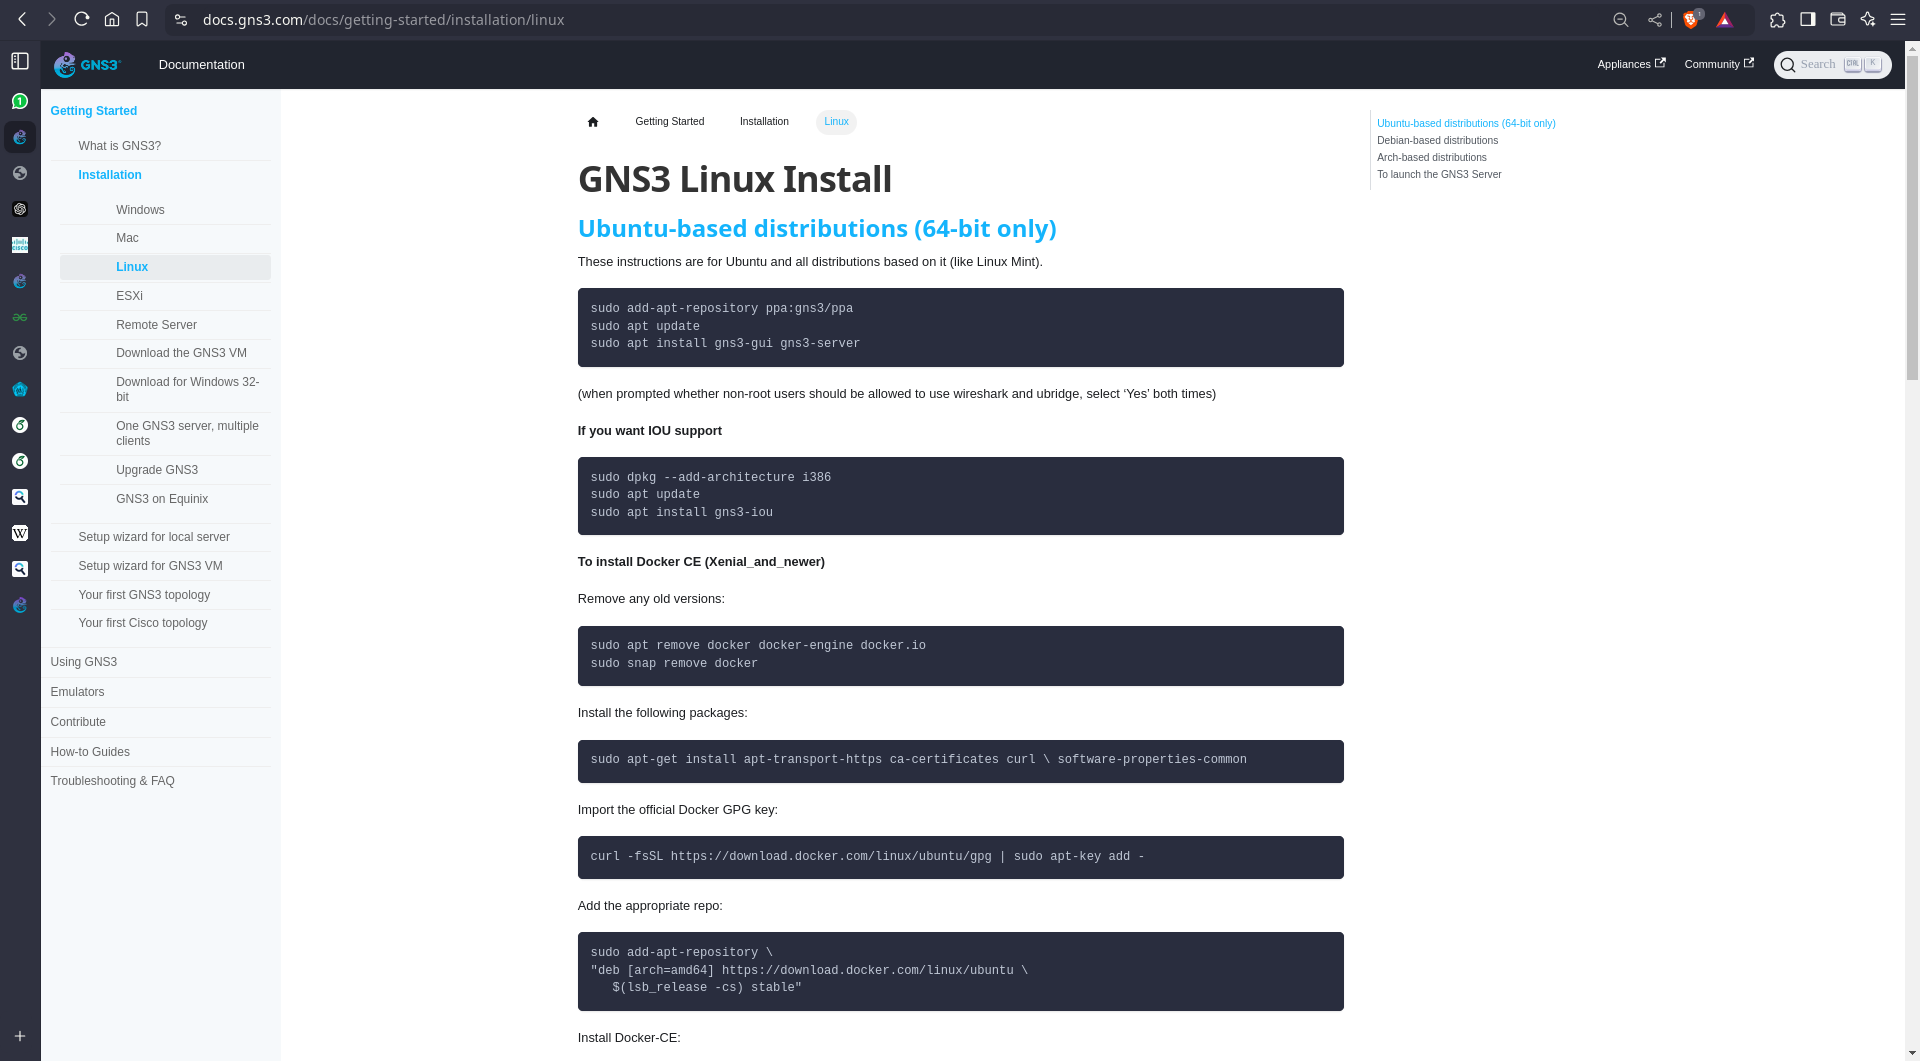
\includegraphics[scale=0.12]{LINUXINSTALLMANUAL.png}
          \caption{\small{Halaman Dokumentasi Instalasi di Linux}}
      \end{figure}

      Didalam halaman dokumentasi linux, akan diberi langkah-langkah untuk 
      dapat menginstal GNS-3 di berbagai distro linux.

      Namun, untuk Fedora Linux, di halaman unduh GNS-3 tidak akan ditemui penjelasan
      tentang instalasi, namun untungnya di dalam repository fedora sudah disediakan
      binary nya siap untuk diinstall.

      \begin{figure}[h]
          \centering
          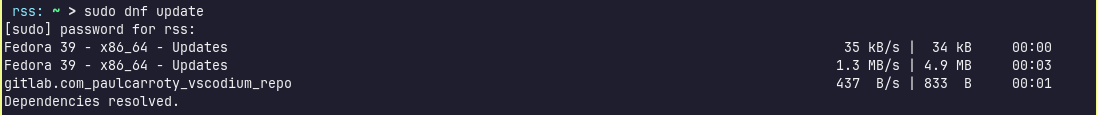
\includegraphics[scale=0.15]{FEDORAREPOSYNC.png}
          \caption{\small{Update Repository Fedora Linux}}
      \end{figure}

      Pertama yang perlu dilakukan adalah untuk memastikan apa repository fedora
      perlu update atau pembaruan index, jadi buka terminal bash lalu
      masukan perintah.
      
      \$ sudo dnf update

      Setelah repository telah diperbaruhi, baru bisa dimulai instalasi dengan
      perintah.

      \$ sudo dnf install gns3-server gns3-gui

      Perintah ini akan mengunduh dan menginstall server serta graphical interface,
      GNS-3.
    
      Namun, aplikasi GNS-3 tidak dapat dengan sendirinya mesimulasikan
      sebuah jaringan utuh, memerlukan beberapa komponen tambahan,
      berikut beberapa komponen tersebut dan cara menginstallnya
      di Fedora Linux.

      \begin{enumerate}[label=\arabic*.]
        \item Dynamips

          Untuk menginstal Dynamips di fedora linux dapat dilakukan dengan
          perintah terminal yaitu.

          \$ sudo dnf install dynamips

        \item Wireshark

          Untuk menginstal Wireshark di fedora linux dapat dilakukan dengan
          perintah terminal yaitu.

          \$ sudo dnf install wireshark

        \item VPCS

          VPCS tidak akan ditemui didalam repository fedora linux, dan hanya
          dapat diinstall dengan secara manual melalui repository github
          vpcs.

          Pertama buka halaman repository project vpcs di github yang ada
          pada url, https://github.com/GNS3/vpcs.

          \begin{figure}[h]
              \centering
              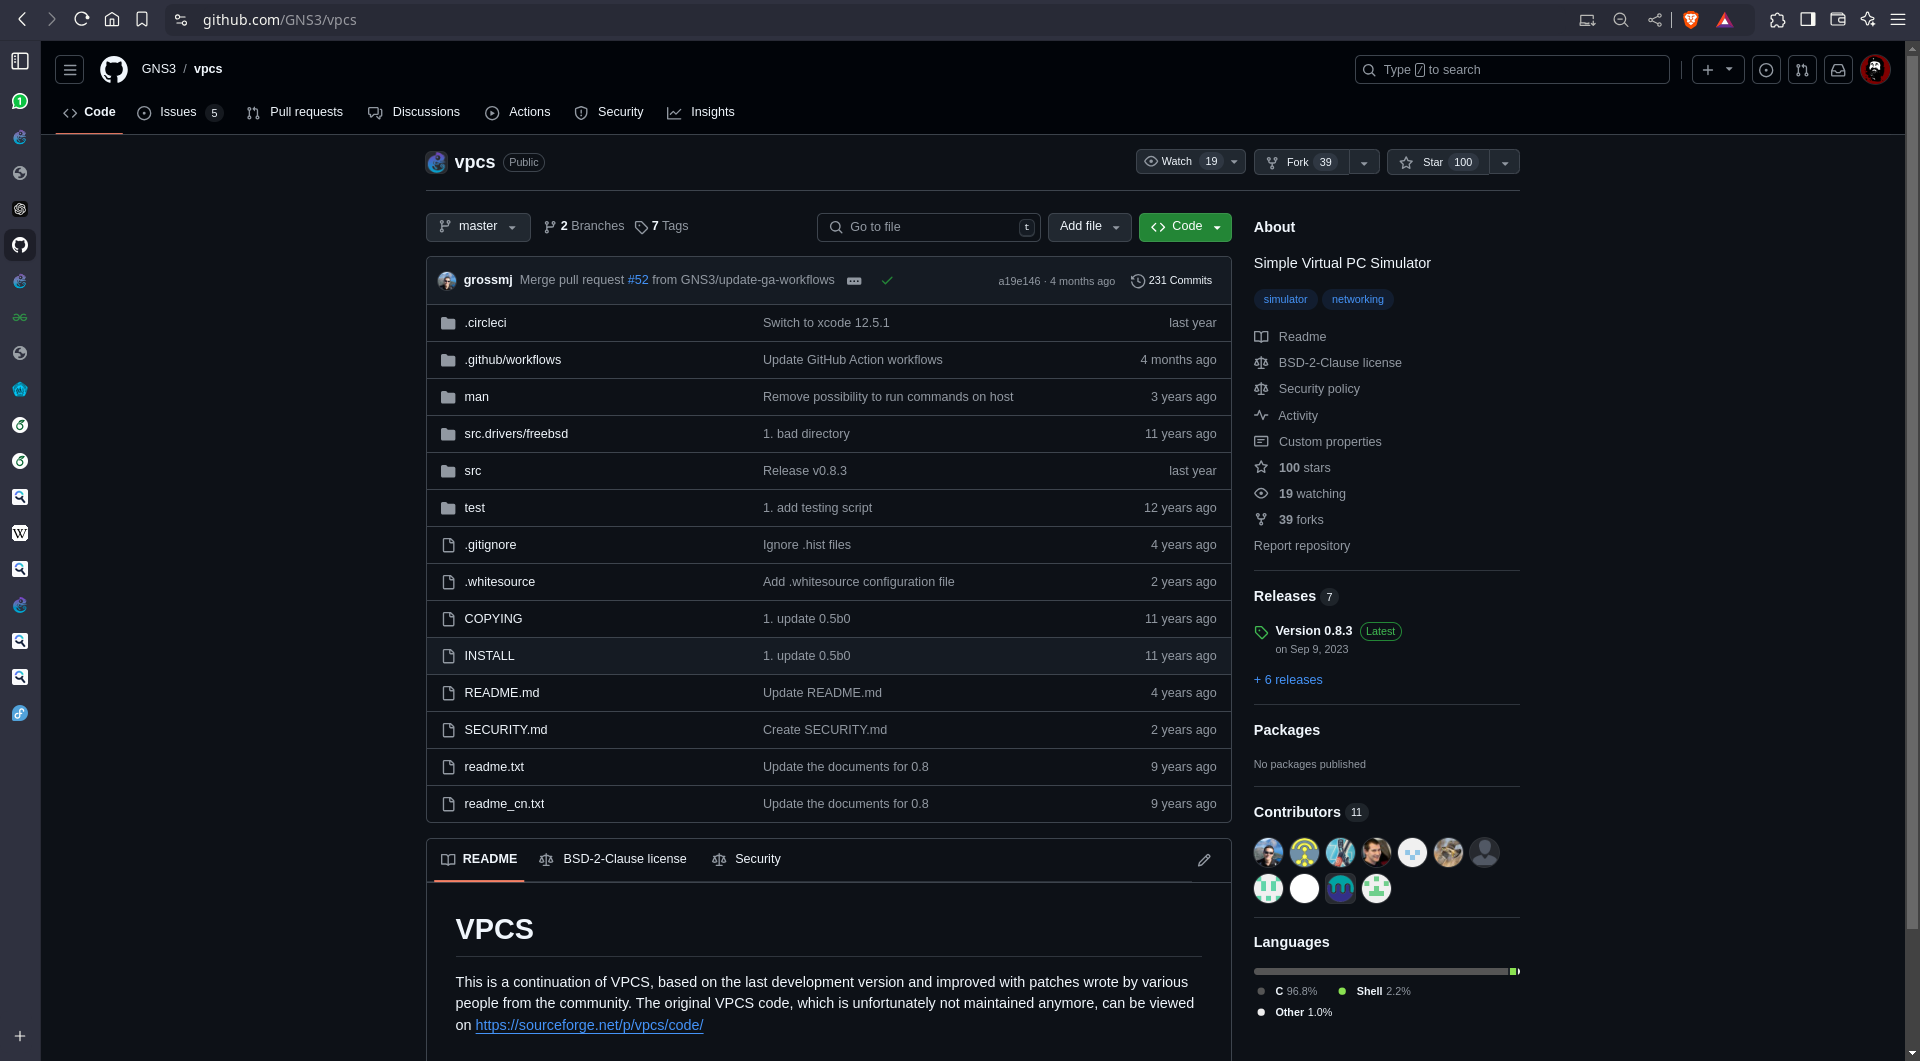
\includegraphics[scale=0.13]{VPCSREPO.png}
              \caption{\small{Halaman Github Project VPCS}}
          \end{figure}

          Lalu dapat diunduh project tersebut melalui opsi download pojok
          kanan atas tepatnya di tombol warna hijau.

          \begin{figure}[h]
              \centering
              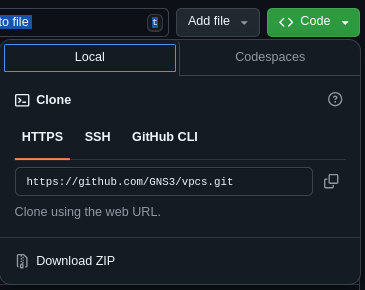
\includegraphics[scale=0.5]{DOWNLOADMENUGIT.png}
              \caption{\small{Opsi Download Repository}}
          \end{figure}

          Atau dengan menggunakan terminal, yaitu dengan perintah git jika telah
          diinstall sebelumnya.

          \$ git clone https://github.com/GNS3/vpcs

          Setelah project telah diinstal, maka perlu dilakukan langkah berikutnya
          yaitu untuk meng-compile program vpcs.

          Tapi sebelum memulai proses kompilasi perlu dipastikan aplikasi-aplikasi
          yang diperlukan seperti kompiler, dan lain sebagainya telah diinstall,
          di fedora linux dapat menggunakan perintah terminal sebagai berikut.

          \$ sudo dnf group install "C Development Tools and Libraries" "Development Tools"

          Lalu setelah menginstall alat-alat yang dibutuhkan, dapat memulai
          proses kompilasi.

          Pertama lakukan 'cd' atau change directory ke dalam folder project
          vpcs yang telah diunduh.

          \$ cd vpcs

          jika dilakukan dengan benar, maka sekarang working directory terminal
          akan berada di dalam folder project vpcs, untuk memastikan dapat
          di lampirkan isi dari folder project tersebut dengan perintah.

          \$ ls -l

          \begin{figure}[h]
              \centering
              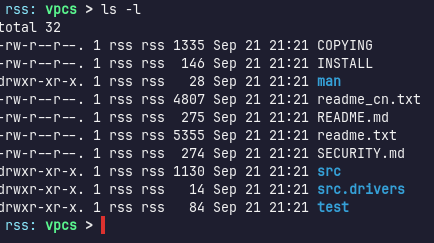
\includegraphics[scale=0.3]{VPCSDIRLS.png}
              \caption{\small{Isi Folder Project VPCS}}
          \end{figure}


          Selanjutnya, 'cd' lagi kedalam folder yang bernama 'src', dengan perintah
          yaitu.

          \$ cd src

          Jika dilakukan perintah 'ls' atau list directory kembali didalam
          folder 'src' ini akan terlihat bahwa folder ini berisikan file-file
          source code dan juga sebuah file script yang executable untuk membuat
          executable vpcs, yaitu 'mk.sh'.


          \begin{figure}[h]
              \centering
              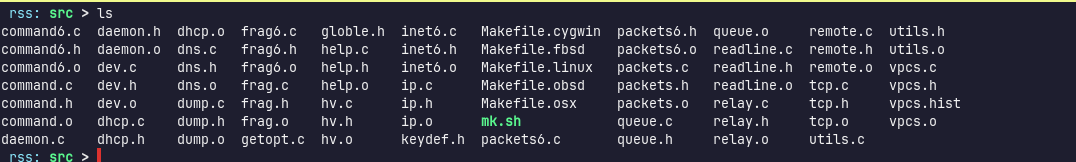
\includegraphics[scale=0.3]{VPCSSRCDIRLS.png}
              \caption{\small{Isi Folder 'src' Project VPCS}}
          \end{figure}


          Yang hanya perlu dilakukan sekarang adalah untuk menjalankan
          script tersebut, didalam terminal ini dapat dilakukan dengan.

          \$ sh mk.sh

          \begin{figure}[h]
              \centering
              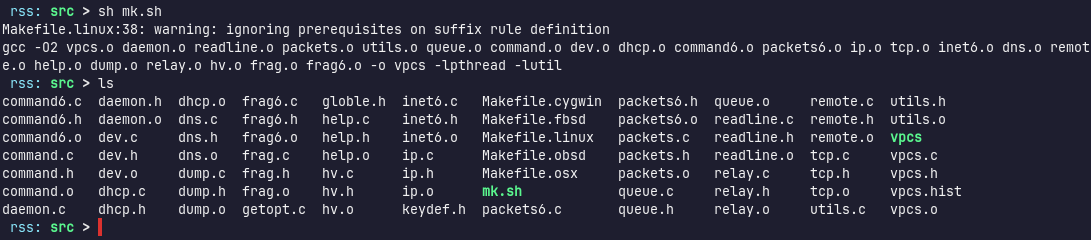
\includegraphics[scale=0.3]{VPCSBUILD.png}
              \caption{\small{Hasil Proses Kompilasi}}
          \end{figure}

          Setelah berhasil untuk di kompile, maka selanjutnya hanya untuk
          meletakan executable vpcs ini di tempat yang sesuai, biasanya
          sistem linux menaruh file-file executable di dua tempat yaitu
          di /usr/bin untuk user root atau admin, dan untuk user di
          .local/bin di path home masing-masing user biasa.

          Jika semua itu telah dilakukan maka GNS-3 akan dapat menemukan executable
          vpcs tersebut.

        \item VirtualBox dan QEMU

          Didalam Fedora Linux, untuk menginstall VirtualBox serta QEMU dapat dengan 
          mudah melalui repository fedora linux, dengan perintah terminal yaitu.

          \$ sudo dnf install VirtualBox QEMU

      \end{enumerate}

\end{document}
